\documentclass[conference]{IEEEtran}
\usepackage{iftex}
\ifPDFTeX
  % pdfLaTeX: cần gói vntex (TeX Live: texlive-lang-other) cho font T5.
  \usepackage[utf8]{inputenc}
  \usepackage[T5]{fontenc}
  \usepackage[vietnamese]{babel}
\else
  % XeLaTeX/LuaLaTeX (khuyên dùng): font Unicode đủ dấu tiếng Việt.
  \usepackage{fontspec}
  \setmainfont{texgyretermes}[
    Extension = .otf,
    UprightFont = *-regular,
    BoldFont = *-bold,
    ItalicFont = *-italic,
    BoldItalicFont = *-bolditalic,
  ]
\fi
\usepackage{amsmath,amssymb}
\usepackage{graphicx}
\usepackage{booktabs}
\usepackage{multirow}
\usepackage[hidelinks]{hyperref}
\graphicspath{{figures/}}

\begin{document}

\title{Deadline-Constrained Multi-UAV Risk Coverage}

\author{\IEEEauthorblockN{Pham Duy Khanh, Nguyen Nho Dung, Duong Tien Dat,
Vu Minh Long, Pham Viet Dung}
\IEEEauthorblockA{Hanoi University of Science and Technology\\
\texttt{\{Khanh.PD261087M, Dung.NN261236M, Dat.DT261265M, Long.VM261264M, Dung.PV261090M\}@sis.hust.edu.vn}}
}
\maketitle

\begin{abstract}
Bài báo này tổng kết bài tập lớn môn Design and Analysis of Algorithms. Nhiệm vụ đặt ra là
điều phối $K=4$ máy bay không người lái (UAV) trên một bản đồ rủi ro dạng lưới, trong đó
mỗi UAV có ngân sách pin riêng và lượng rủi ro quan sát được cần đạt lớn nhất. Về bản chất,
đây là biến thể nhiều ngân sách của bài toán Budgeted Maximum Coverage, một bài toán
NP-hard. Cả bộ thực nghiệm đều xây từ RescueNet, bộ ảnh UAV chụp sau bão Michael kèm mask
phân đoạn 11 lớp: mask được cắt thành lưới $20\times20$, rồi nhóm sinh ra route bay và ngân
sách pin cho từng UAV từ chính lưới đó. Nhóm cài đặt greedy thuần, greedy tỉ lệ kết hợp seed
và tìm kiếm cục bộ, cộng thêm một thuật toán đề xuất có xét pin riêng từng UAV; mọi kết quả
đều đối chứng với quy hoạch số nguyên (ILP) và được validator độc lập tính lại từ đầu. Trên
45 thực thể OR-Library, greedy tỉ lệ có seed và tìm kiếm cục bộ đạt 99,4--99,7\,\% nghiệm
tối ưu, trong khi greedy thuần chỉ đạt 40,8--43,5\,\%. Trên 350 ảnh RescueNet nhân 4 mức
ngân sách, thuật toán đề xuất đạt trung bình 0,971--0,984 lần nghiệm ILP, hơn baseline ngân
sách chung từ 4,3 đến 6,2 điểm phần trăm (Wilcoxon ghép cặp cho $p < 10^{-44}$ ở cả bốn
mức). Mỗi lần giải chỉ mất khoảng 46\,ms, trong khi ILP cần từ 3,2 đến 66,2\,giây. Bài báo
cũng có ablation từng thành phần, khảo sát độ nhạy và phân tích thời gian chạy.
\end{abstract}

\begin{IEEEkeywords}
coverage path planning, Budgeted Maximum Coverage, tối ưu hóa submodular, multi-UAV,
RescueNet, quy hoạch số nguyên
\end{IEEEkeywords}

\section{Giới thiệu}
% Nguồn: README.md "Mô tả chung" + "Bài toán và khái niệm nền"; docs/mo-hinh-du-lieu.md
Đề tài là bài tập lớn môn Design and Analysis of Algorithms, và toàn bộ dữ liệu của nhóm
xoay quanh một bộ ảnh thật: RescueNet~\cite{rescuenet}, gồm 449 ảnh UAV chụp sau bão Michael
(10/2018), mỗi ảnh kèm mask phân đoạn hư hại 11 lớp. Bài tập xét trường hợp sử dụng bốn UAV để quan sát các khu vực có mức độ hư hại khác nhau. Do ngân sách pin của từng UAV bị giới hạn, nhóm không đặt mục tiêu quan sát toàn bộ khu vực. Thay vào đó, bài toán cần lựa chọn các route sao cho tổng điểm rủi ro được phủ là lớn nhất, đồng thời không vượt quá ngân sách pin của mỗi UAV.

Để thuật toán giải được, nhóm cắt mỗi ảnh thành lưới $20\times20$ ô; ô có hư hại nặng
nhận điểm rủi ro cao, tính thẳng từ mask. Mỗi UAV có một ngân sách pin riêng và đi được một
số route; mỗi route phủ một tập ô với chi phí pin xác định. Chọn tập route tối đa hóa tổng
rủi ro được phủ là biến thể nhiều ngân sách của bài toán Budgeted Maximum Coverage,
NP-hard~\cite{khuller1999}, nên nhóm đi theo hướng heuristic và đánh giá đối chứng bằng
ILP thay vì tìm lời giải chính xác. Công việc chia thành hai pha: pha 1 kiểm chứng thuật
toán trên 45 thực thể OR-Library với một ngân sách chung, pha 2 chạy trên bản đồ rủi ro xây
từ RescueNet với ngân sách riêng từng UAV (hình~\ref{fig:pipeline}).
\begin{figure*}[!t]
\centering
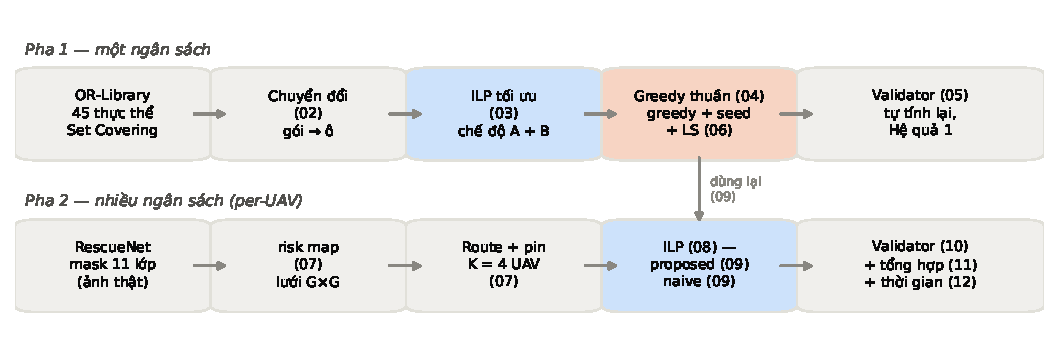
\includegraphics[width=\textwidth]{h1_pipeline.pdf}
\caption{Quy trình hai pha của dự án. Xanh = nghiệm đối chứng ILP; cam = heuristic.
Số trong ngoặc là thứ tự script trong \texttt{pipeline/}; mọi nghiệm đều đi qua
validator độc lập trước khi vào bảng số liệu.}
\label{fig:pipeline}
\end{figure*}


Cụ thể, nhóm đã làm bốn mảng việc:
\begin{itemize}
\item Quy trình xây dựng bộ thực nghiệm từ dữ liệu thật: chuyển mask phân đoạn của bộ dữ
liệu RescueNet~\cite{rescuenet} thành bản đồ rủi ro dạng lưới, sinh route và ngân sách pin
cho $K=4$ UAV, cho ra 350 thực thể (instance) đủ điều kiện trên tập validation. Toàn bộ quy
trình có mã nguồn, kiểm thử (82 test pytest) và tài liệu trong repo của nhóm.
\item Thuật toán đề xuất: greedy tỉ lệ lazy (kỹ thuật CELF~\cite{leskovec2007}) xét ngân
sách riêng từng UAV, kết hợp nghiệm gói đơn tốt nhất, đa hóa bằng seed và tìm kiếm cục bộ
drop-and-refill.
\item Đánh giá đối chứng với ILP: 45 thực thể OR-Library ở pha 1 và 1400 lần giải trên 350
ảnh RescueNet ở pha 2; kết quả được bộ validator độc lập tự tính lại từ dữ liệu đầu vào,
không dùng số liệu thuật toán tự báo cáo.
\item Phân tích: ablation từng thành phần, kiểm định Wilcoxon ghép cặp, khảo sát độ nhạy
với bảng điểm rủi ro và kích thước lưới, cùng phân tích thời gian chạy lý thuyết và đo
thực tế.
\end{itemize}

\textbf{Phạm vi mô hình.} Đề tài gốc nêu ràng buộc deadline; trong khuôn khổ này, ràng buộc
thời gian được mô hình hóa dưới dạng ngân sách năng lượng (chi phí của route tương ứng thời
gian bay/pin) cho từng UAV. Việc bổ sung mốc thời gian riêng cho từng ô là hướng phát triển
(mục~\ref{sec:conclusion}). Ngoài ra, route, pin và số UAV là \emph{mô hình tổng hợp do nhóm
thiết kế} dựa trên dữ liệu nhãn thật của RescueNet; bản đồ rủi ro mới là phần dựa trực tiếp
vào dữ liệu thật. Nhóm nêu rõ điều này ở mục~\ref{sec:discussion}.

\section{Công trình liên quan}
% Nguồn: docs/greedy-ls-thiet-ke.md mục 9; README "Bảo đảm xấp xỉ"
\textbf{Tối đa hóa coverage có ngân sách.} Budgeted Maximum Coverage là bài toán kinh điển
của tối ưu hóa submodular với ràng buộc knapsack. Cho trường hợp một ngân sách, Khuller, Moss
và Naor~\cite{khuller1999} kết hợp greedy theo tỉ lệ với nghiệm gói đơn tốt nhất; thuật toán
này bảo đảm $\tfrac{1}{2}(1-1/e) \approx 0{,}32$ so với tối ưu. Cận $1-1/e \approx 0{,}63$
khó đạt hơn nhiều: nó chỉ đúng khi mọi gói cùng chi phí
(Nemhauser--Wolsey--Fisher~\cite{nemhauser1978}), hoặc khi duyệt mọi bộ ba gói đầu tiên
(Sviridenko~\cite{sviridenko2004}). Cách sau không khả thi với số gói từ 1000 trở lên như
trong thực thể của nhóm. Trường hợp \emph{nhiều ngân sách} (mỗi UAV một pin) thì chưa rõ:
nhóm chưa kiểm chứng được cận xấp xỉ nào trong tài liệu cho trường hợp này. Vì vậy bài báo
không khẳng định thuật toán ở mục~\ref{sec:algorithm} có bảo đảm lý thuyết; đánh giá thuần
thực nghiệm so với nghiệm ILP.

\textbf{Phạm vi khảo sát.} Bài báo tiếp cận đề tài từ góc độ tối ưu hóa combinatorial. Các
khía cạnh planning đường bay vật lý (động học, tránh va chạm, địa hình) và khảo sát hệ thống
tài liệu coverage path planning cho UAV nằm ngoài phạm vi của bài tập lớn.

\textbf{Bộ dữ liệu RescueNet.} Rahnemoonfar, Chowdhury và Murphy~\cite{rescuenet} công bố bộ
dữ liệu ảnh UAV độ phân giải cao chụp sau bão Michael (10/2018) kèm mask phân đoạn 11 lớp
(nhãn 0--10). Đây là nguồn nhãn thật duy nhất mà nhóm dùng để xây dựng bản đồ rủi ro.

\section{Bài toán và mô hình hóa}
\label{sec:model}
% Nguồn: README "Bài toán và khái niệm nền"; docs/mo-hinh-du-lieu.md; docs/phase2-rescuenet-thiet-ke.md

\subsection{Budgeted Maximum Coverage}
Cho một universe gồm $m$ ô và $n$ gói; gói $j$ có chi phí $c_j > 0$ và phủ một tập ô
$S_j \subseteq \{1,\dots,m\}$. Cần chọn tập gói $X$ sao cho
\begin{equation}
\max_{X} \; f(X) = \Bigl| \bigcup_{j \in X} S_j \Bigr|
\quad\text{sao cho}\quad \sum_{j \in X} c_j \le B ,
\label{eq:bmc}
\end{equation}
trong đó các ô bị phủ nhiều lần chỉ tính một lần. Ở dạng có trọng số (Pha 2), hàm mục tiêu
là $ \sum_{i \in \bigcup_{j \in X} S_j} w_i $ với $w_i$ là điểm rủi ro của ô $i$. Đây là bài
toán NP-hard (quy về từ Set Cover~\cite{khuller1999}).

\subsection{Mô hình đa UAV với ngân sách pin riêng}
\label{sec:uavmodel}
Pha 2 mở rộng~\eqref{eq:bmc} như sau. Hệ gồm $K = 4$ UAV; UAV $u$ có ngân sách pin $B_u$.
Thang ngân sách lấy từ chi phí tham chiếu $R$: chi phí nhỏ nhất để phủ hết mọi ô có điểm
dương, tính bằng ILP phủ trọn (mục~\ref{sec:setup}). Mỗi route $j$ được gán trước cho một
UAV $u(j)$; chỉ UAV đó mới được chọn route này. Gọi $X_u$ là tập route UAV $u$ được chọn,
ràng buộc trở thành $\sum_{j \in X_u} c_j \le B_u$ với mọi $u$.
Thuật toán tối ưu đối chứng là ILP sau (giải bằng CBC~\cite{cbc} qua PuLP~\cite{pulp}):
\begin{align}
\max_{x_j \in \{0,1\}} \quad & \sum_{i=1}^{m} w_i \, y_i \notag \\
\text{sao cho} \quad & y_i \le \textstyle\sum_{j:\, i \in S_j} x_j, && \forall i \notag \\
& \textstyle\sum_{j:\, u(j)=u} c_j x_j \le B_u, && \forall u. \label{eq:ilp}
\end{align}
Có một hệ quả đơn giản nhưng hữu ích để bắt lỗi: nếu $B < R$ thì không thể phủ 100\,\% các ô
điểm dương. Lý do: một nghiệm phủ hết với chi phí $\le B < R$ chính là lời giải phủ trọn rẻ
hơn $R$, mâu thuẫn với định nghĩa $R$. Bộ validator (mục~\ref{sec:setup}) dựa trên hệ quả
này để phát hiện bug.

\subsection{Từ ảnh RescueNet sang thực thể bài toán}
Mỗi ảnh được raster hóa thành lưới $G \times G$, mặc định $G=20$ (tối đa $m = 400$ ô). Điểm
rủi ro của một ô lấy trung bình điểm rủi ro của các pixel mask trong ô đó. Bảng ánh xạ 11
nhãn $\to$ điểm rủi ro đặt theo nguyên tắc: hư hại nặng thì điểm cao, ví dụ
\emph{Building--Total-Destruction} hay \emph{Road--Blocked}. Từ lưới, pipeline sinh các
route tự tránh (self-avoiding) xuất phát từ các điểm cố định của $K$ UAV, lệch về ô có rủi ro cao. Chi phí route tỷ lệ độ dài. Ngân sách của UAV $u$ là $B_u = \lfloor \text{mức\%} \times R \times s_u \rfloor$,
trong đó $s_u$ là hệ số riêng của từng UAV, ngẫu nhiên trong khoảng $\pm 20\,\%$ quanh
giá trị bằng nhau (chốt trong tài liệu thiết kế kèm mã nguồn). Lý do của từng lựa chọn (kích thước lưới, bảng điểm, cách chọn
ảnh, công thức ngân sách) nằm trong tài liệu thiết kế kèm mã nguồn
(\texttt{docs/phase2-rescuenet-thiet-ke.md}). Không phải ảnh nào cũng dùng được: chỉ các
ảnh có ít nhất 60 ô điểm dương được giữ lại (350/449 ảnh validation); 99 ảnh bị loại vì quá
ít ô để phủ.

\section{Thuật toán}
\label{sec:algorithm}
% Nguồn: docs/greedy-thuan-thiet-ke.md; docs/greedy-ls-thiet-ke.md; proposed-algorithm/README.md

\subsection{Baseline}
\textbf{Greedy thuần} (Pha 1) chọn gói phủ nhiều ô mới nhất, lặp cho đến khi hết ngân sách.
Thuật toán này \emph{không} có bảo đảm xấp xỉ khi các gói chi phí khác nhau. Thực nghiệm
(mục~\ref{sec:results}) cho thấy nó kém xa tối ưu. \textbf{Naive} (Pha 2) làm đơn giản hơn:
chạy greedy trên ngân sách chung $\sum_u B_u$, rồi sửa vi phạm pin bằng cách bỏ route và lấp
lại chỗ trống. Đây chính là cách làm thiếu cân nhắc đến ngân sách riêng từng UAV, giữ lại
làm mốc so sánh.

\subsection{Thuật toán đề xuất}
Thuật toán đề xuất, nhóm gọi tắt là \emph{proposed}, ghép bốn thành phần:
\begin{enumerate}
\item \textbf{Greedy tỉ lệ lazy theo từng UAV:} mỗi bước, với UAV $u$ còn dư pin, chọn route
tối đa tỉ lệ $\lvert S_j \setminus \text{đã phủ} \rvert / c_j$ trong các route của $u$. Để
đỡ tốn tính toán, ta dùng kỹ thuật lazy evaluation (CELF~\cite{leskovec2007}): danh sách
ứng viên được giữ theo giá trị cũ và chỉ tính lại khi giá trị cũ không còn đứng đầu. Số phép
đánh giá nhờ vậy giảm mạnh.
\item \textbf{Gói đơn tốt nhất:} so sánh nghiệm greedy với route đơn có $f(\{j\})$ lớn nhất,
lấy giá trị cao hơn (bố cục của Khuller--Moss--Naor~\cite{khuller1999}).
\item \textbf{Đa hóa bằng seed:} khởi tạo thứ tự ưu tiên của các route theo nhiều tiêu chí
(20 route phủ nhiều nhất, 20 route tỉ lệ tốt nhất, ...) và chạy lại greedy từ mỗi seed,
giữ nghiệm tốt nhất.
\item \textbf{Tìm kiếm cục bộ drop-and-refill:} thử bỏ từng route đã chọn và lấp chỗ trống
bằng greedy tỉ lệ, lặp đến khi không cải thiện.
\end{enumerate}
Mọi bước đều kiểm tra ràng buộc pin của từng UAV. Với cấu hình mặc định, thuật toán
deterministic. Phân tích Big-O nằm trong tài liệu kỹ thuật của nhóm
(\texttt{docs/phase2-thoi-gian-chay.md}); mục~\ref{sec:results} tóm tắt số đo thời gian.

\section{Thiết lập thực nghiệm}
\label{sec:setup}
% Nguồn: README "Cài đặt và chạy"; docs/ilp-solver-thiet-ke.md; docs/phase2-rescuenet-thiet-ke.md
\textbf{Pha 1 (OR-Library, một ngân sách).} 45 thực thể Set Covering (bộ 4, 5, 6, A--D)
lấy từ OR-Library~\cite{beasley1990}. Ngân sách đặt theo nghiệm tối ưu phủ trọn OPT:
$B = \lfloor \text{mức\%} \times \mathrm{OPT} \rfloor$ với mức 75/50/25\,\%. Bảng OPT lấy từ
Ohlsson và cộng sự~\cite{ohlsson1999} (số liệu gốc Beasley~\cite{beasley1990}); nhóm đã tái
lập lại cả 45 giá trị bằng ILP và khớp hết. Mỗi cặp (thực thể, mức) tính là một lần giải,
vậy mỗi heuristic có 135 lần giải.

\textbf{Pha 2 (RescueNet, nhiều ngân sách).} Dữ liệu lấy từ tập validation RescueNet
(449 ảnh). Kết quả chính chạy trên toàn bộ 350 ảnh đủ điều kiện với lưới $20\times20$, bảng
điểm mặc định và $K=4$ UAV. Mỗi thuật toán phải giải 1400 lần, tức 350 ảnh nhân 4 mức ngân
sách (25/50/75/100\,\% của $R$, chia thành $B_u$ cho từng UAV). Thực thể có $m$ dao động từ
61 đến 400 (trung bình 174), còn $n$ từ 251 đến 1097 (trung bình 719).

\textbf{Tiêu chí đánh giá} gồm ba phần: (i) tỉ lệ objective của thuật toán so với objective
của ILP trên cùng thực thể và mức; (ii) số ca thắng/hòa/thua theo thực thể (dung sai
$10^{-9}$), kèm kiểm định Wilcoxon ghép cặp hai phía; (iii) thời gian chạy. ILP bị giới hạn
120\,giây. Các ca CBC hết giờ được ghi là \emph{best-known}: 393/1400 ca ở lần chạy 350 ảnh,
chủ yếu ở $m$ lớn và mức ngân sách cao. Với các ca này, tỉ lệ là so với nghiệm tốt nhất ILP
tìm được, và \emph{có thể lớn hơn 1}.

\textbf{Validator độc lập.} Validator không tin số liệu thuật toán tự báo cáo. Nó tự tính
lại chi phí và coverage từ danh sách route đã chọn, rồi đối chiếu với ràng buộc ngân sách,
số liệu khai báo, và bất biến ở mục~\ref{sec:uavmodel}. Thấy sai lệch là báo lỗi và thoát
với mã khác 0. Lần chạy 350 ảnh: 8400 file kết quả, không có lỗi nào.

\begin{figure*}[!t]
\centering
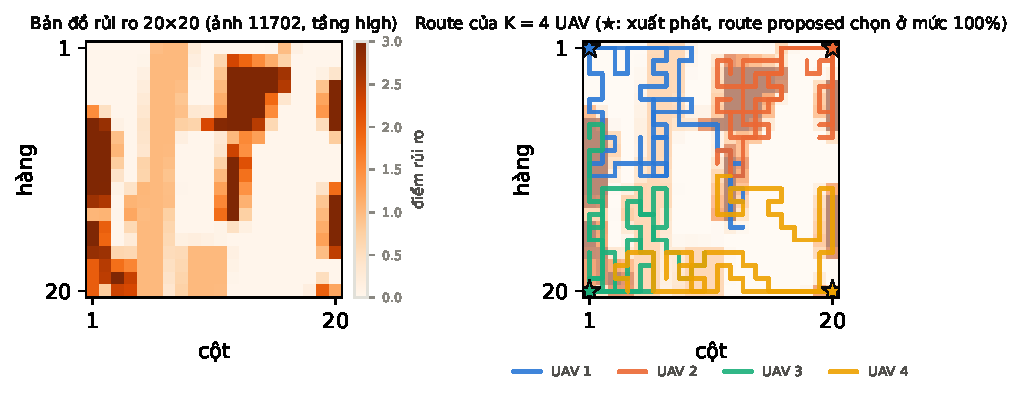
\includegraphics[width=\textwidth]{h2_example_instance.pdf}
\caption{Minh họa một thực thể trên ảnh tầng hư hại cao (ảnh 11702). Trái: bản đồ
rủi ro $20\times20$ trích từ mask RescueNet (nhãn là dữ liệu thật). Phải: các route
của $K=4$ UAV (★: điểm xuất phát ở 4 góc) mà thuật toán đề xuất chọn ở mức ngân
sách 100\,\%, phủ tập trung lên vùng rủi ro cao; lưới, route và pin là mô hình
tổng hợp của nhóm.}
\label{fig:example}
\end{figure*}

\section{Kết quả thực nghiệm}
\label{sec:results}
% Nguồn: docs/phase2-ket-qua.md; docs/phase2-thoi-gian-chay.md; số Pha 1 tính từ data/results/
% (lệnh tổng hợp được ghi trong tài liệu dự án; việc chuẩn hóa thành script là việc C1 trong
% report/ke-hoach-bo-sung-paper.md)

\subsection{Pha 1: OR-Library}
\begin{figure}[!t]
\centering
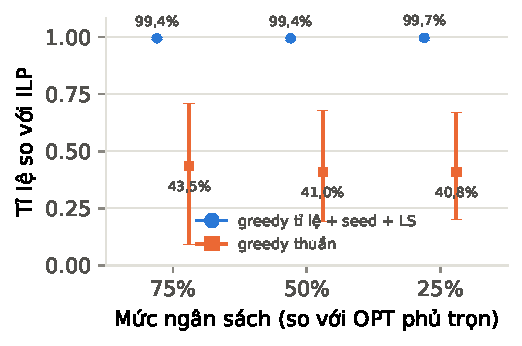
\includegraphics[width=\columnwidth]{h5_phase1_results.pdf}
\caption{Pha 1 (OR-Library, 45 thực thể): tỉ lệ so với nghiệm ILP tối ưu
(điểm: trung bình, gạch dọc: khoảng min--max). Greedy thuần (cam) đạt trung bình
chỉ 40,8--43,5\,\%; greedy tỉ lệ + seed + tìm kiếm cục bộ (xanh) đạt
99,4--99,7\,\%.}
\label{fig:phase1}
\end{figure}
Bảng~\ref{tab:phase1} và hình~\ref{fig:phase1} tóm tắt 135 lần giải mỗi heuristic. Cả 45 ca
ILP đều đạt \texttt{optimal}. Greedy thuần chỉ đạt trung bình 40,8--43,5\,\% nghiệm tối ưu;
phân tích ở mục~\ref{sec:algorithm} đã báo trước điều này: greedy theo số ô mới không phù
hợp với bài toán có chi phí. Thuật toán greedy tỉ lệ kết hợp seed và tìm kiếm cục bộ thì
khác hẳn: 99,4--99,7\,\% trung bình, thấp nhất 98,5\,\%, thời gian không quá 64\,ms mỗi lần
giải.

\begin{table}[!t]
\centering
\caption{Pha 1 (OR-Library, 45 thực thể $\times$ 3 mức): tỉ lệ so với nghiệm ILP tối ưu.}
\label{tab:phase1}
\begin{tabular}{lccc}
\toprule
 & 75\,\% & 50\,\% & 25\,\% \\
\midrule
Greedy thuần & 0{,}435 & 0{,}410 & 0{,}408 \\
Greedy tỉ lệ + seed + LS & \textbf{0{,}994} & \textbf{0{,}994} & \textbf{0{,}997} \\
\midrule
\multicolumn{4}{l}{\footnotesize Thời gian TB: greedy thuần 1,6--4,5\,ms; greedy+seed+LS 26--64\,ms.}\\
\multicolumn{4}{l}{\footnotesize Tỉ lệ $=$ objective heuristic / objective ILP (n $=$ 45 mỗi ô).}\\
\bottomrule
\end{tabular}
\end{table}

\subsection{Pha 2: RescueNet, 350 ảnh}
Hình~\ref{fig:example} minh họa một thực thể hoàn chỉnh. Kết quả chính ở bảng~\ref{tab:phase2}:
trung bình trên 350 ảnh $\times$ 4 mức, tức 1400 lần giải mỗi thuật toán. Trong đó ILP cho
1007 ca \texttt{optimal} và 393 ca \texttt{best-known}. Thuật toán đề xuất đạt 0,971--0,984
lần ILP, hơn naive 4,3--6,2 điểm phần trăm ở mọi mức.

\begin{table}[!t]
\centering
\caption{Pha 2 (350 ảnh): tỉ lệ so với ILP, trung bình (nhỏ nhất).}
\label{tab:phase2}
\begin{tabular}{lcccc}
\toprule
Mức & 25\,\% & 50\,\% & 75\,\% & 100\,\% \\
$n$ & 349 & 350 & 350 & 350 \\
\midrule
Proposed & 0{,}984 & 0{,}971 & 0{,}973 & 0{,}984 \\
         & (0{,}882) & (0{,}862) & (0{,}890) & (0{,}905) \\
Naive    & 0{,}933 & 0{,}908 & 0{,}921 & 0{,}941 \\
         & (0{,}369) & (0{,}659) & (0{,}672) & (0{,}694) \\
\bottomrule
\end{tabular}
\end{table}

\begin{figure}[!t]
\centering
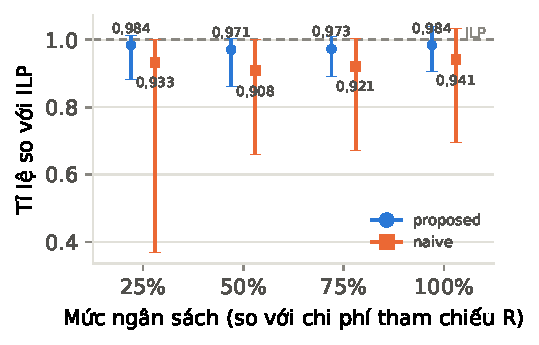
\includegraphics[width=\columnwidth]{h3_main_results.pdf}
\caption{Kết quả chính trên 350 ảnh: tỉ lệ so với ILP (điểm: trung bình,
gạch dọc: khoảng min--max theo thực thể). Các ca ILP \emph{best-known} (28\,\%)
làm tỉ lệ có thể vượt 1; ở đây không ca proposed nào vượt ILP đã chứng minh
tối ưu.}
\label{fig:main}
\end{figure}

Bảng~\ref{tab:wlt} trình bày số lần proposed thắng, hòa và thua naive theo từng mức
ngân sách. Ở mức 25\,\%, proposed thắng 265 trường hợp, hòa 83 và thua 1. Khi ngân sách
tăng lên 100\,\%, số trường hợp tương ứng là 334, 1 và 15. Kiểm định Wilcoxon ghép cặp
cho giá trị $p$ nhỏ hơn $10^{-44}$ ở cả bốn mức. Không có ca nào vượt ILP đã chứng minh
tối ưu (validator kiểm tra toàn bộ). Hình~\ref{fig:main} vẽ lại tỉ lệ của hai thuật toán
kèm khoảng min--max theo thực thể.

\begin{table}[!t]
\centering
\caption{Proposed so với naive theo thực thể (thắng/hòa/thua) và Wilcoxon ghép cặp, 350 ảnh.}
\label{tab:wlt}
\begin{tabular}{lcc}
\toprule
Mức & Thắng/hòa/thua & $p$ (Wilcoxon) \\
\midrule
25\,\% & 265 / 83 / 1 & $4{,}5 \times 10^{-45}$ \\
50\,\% & 321 / 23 / 6 & $8{,}2 \times 10^{-55}$ \\
75\,\% & 333 / 6 / 11 & $1{,}3 \times 10^{-56}$ \\
100\,\% & 334 / 1 / 15 & $3{,}9 \times 10^{-57}$ \\
\bottomrule
\end{tabular}
\end{table}

\subsection{Ablation}
Bảng~\ref{tab:ablation} bỏ từng thành phần của thuật toán đề xuất, trên cùng 350 ảnh. Bỏ
seed mất chất lượng nhiều hơn bỏ tìm kiếm cục bộ. Riêng việc xét pin từng UAV khi chọn
(ratio-only) chỉ hơn naive 0,9--1,4 điểm phần trăm. Nghĩa là phần lớn cải thiện đến từ seed
và tìm kiếm cục bộ, không phải từ việc đổi cách xét ngân sách. Mọi khác biệt đều có
$p < 10^{-18}$ (Wilcoxon).

\begin{table}[!t]
\centering
\caption{Ablation trên 350 ảnh: tỉ lệ trung bình so với ILP.}
\label{tab:ablation}
\begin{tabular}{lcccc}
\toprule
Biến thể & 25\,\% & 50\,\% & 75\,\% & 100\,\% \\
\midrule
Chỉ ratio per-UAV & 0{,}946 & 0{,}919 & 0{,}930 & 0{,}955 \\
Không seed & 0{,}959 & 0{,}937 & 0{,}945 & 0{,}967 \\
Không tìm kiếm cục bộ & 0{,}979 & 0{,}963 & 0{,}967 & 0{,}981 \\
\textbf{Đầy đủ (proposed)} & \textbf{0{,}984} & \textbf{0{,}971} & \textbf{0{,}973} & \textbf{0{,}984} \\
\midrule
Naive & 0{,}933 & 0{,}908 & 0{,}921 & 0{,}941 \\
\bottomrule
\end{tabular}
\end{table}

\subsection{Khảo sát độ nhạy}
Trên 30 ảnh phân tầng, nhóm thử đổi bảng điểm (tree/convex/damage-only) và giảm lưới còn
$10\times10$. Thứ tự proposed $\ge$ naive giữ nguyên ở mọi mức về trung bình. Một ngoại lệ: lưới $10\times10$ ở mức 25\,\%, hai thuật toán gần như bằng nhau ($p = 0{,}32$,
không khác biệt đáng kể). ILP ở cấu hình tree yếu rõ (56/120 ca best-known), nên
gap ở đó là so với best-known chứ không phải tối ưu; tỉ lệ $>1$ (lớn nhất 1{,}016) cũng
xảy ra đúng ở các ca đó.

\subsection{Thời gian chạy}
Số liệu ở bảng~\ref{tab:time}: thuật toán đề xuất mất trung bình 46\,ms mỗi lần giải, tổng
khoảng 65 giây cho cả 1400 lần. ILP thì khác hẳn: 3,2--66,2\,giây trung bình tùy mức ngân
sách, tổng 16,7 giờ CPU. Chất lượng theo số seed (hình~\ref{fig:seeds}) bão hòa rất nhanh:
5 seed đã cho phần lớn cải thiện; tăng từ 20 lên 80 seed chỉ thêm khoảng 0,3--0,5 điểm phần
trăm, đổi lại tốn thêm 87\,ms. Mặc định 20 seed là điểm thỏa hiệp, chưa được tối ưu hóa:
giảm còn 10 seed bớt khoảng 41\,\% thời gian, mất 0,2--0,6 điểm. Thời gian một lần giải tăng
gần tuyến tính theo số route $n$ (hệ số mũ log--log 1,06) và gần như không phụ thuộc số ô
$m$ (hình~\ref{fig:scale}).

\begin{table}[!t]
\centering
\caption{Thời gian trung bình mỗi lần giải, lần chạy 350 ảnh (1400 ca/thuật toán).}
\label{tab:time}
\begin{tabular}{lcc}
\toprule
Thuật toán & TB & Lớn nhất \\
\midrule
Proposed & 46{,}4\,ms & 245\,ms \\
Naive & 66{,}5\,ms & 294\,ms \\
ILP (theo mức 25/50/75/100\,\%) & 3,2 / 42,2 / 60,0 / 66,2\,s & $\ge$ 120\,s (giới hạn) \\
\bottomrule
\end{tabular}
\end{table}

\begin{figure}[!t]
\centering
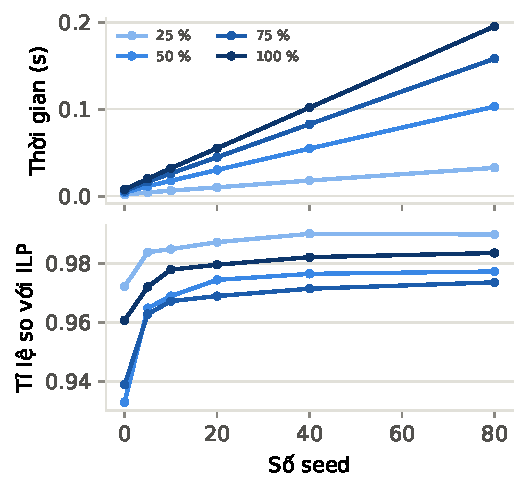
\includegraphics[width=\columnwidth]{h4_seeds_quality_time.pdf}
\caption{Chất lượng--thời gian theo số seed (30 ảnh, trung bình). Trên: thời gian
tăng gần tuyến tính theo số seed. Dưới: 5 seed đã cho phần lớn cải thiện; từ 20 lên
80 seed tỉ lệ chỉ thêm khoảng 0,3--0,5 điểm phần trăm.}
\label{fig:seeds}
\end{figure}

\begin{figure}[!t]
\centering
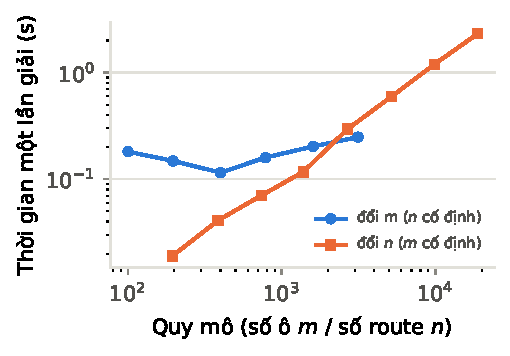
\includegraphics[width=\columnwidth]{h6_scale.pdf}
\caption{Thời gian một lần giải của thuật toán đề xuất theo quy mô thực thể
(thang log--log): tăng theo số route $n$ với $m$ cố định, gần phẳng theo số ô
$m$ với $n$ cố định.}
\label{fig:scale}
\end{figure}

\section{Thảo luận và hạn chế}
\label{sec:discussion}
% Nguồn: docs/phase2-ket-qua.md mục 5; docs/phase2-rescuenet-thiet-ke.md mục 0
\begin{enumerate}
\item \textbf{Thực thể tổng hợp.} Chỉ bản đồ rủi ro dựa trên nhãn thật của RescueNet;
route, pin, $K=4$ và công thức ngân sách do nhóm thiết kế. RescueNet không có khái niệm
UAV, pin hay đáp án tối ưu.
\item \textbf{Ràng buộc thời gian.} Đề tài nêu deadline; mô hình hiện tại dùng ngân sách
năng lượng từng UAV. Deadline thời gian riêng cho từng ô là hướng mở rộng.
\item \textbf{ILP không luôn tối ưu.} 28\,\% ca (393/1400) chỉ best-known sau 120\,giây,
tập trung ở $m$ lớn và mức ngân sách cao; tỉ lệ ở các ca đó có thể vượt 1.
\item \textbf{Lựa chọn ảnh.} Kết quả chính dùng mọi ảnh có $\ge 60$ ô điểm dương (350/449);
99 ảnh bị loại. Chỉ dùng tập validation, chưa có tập kiểm định độc lập.
\item \textbf{Bảo đảm lý thuyết.} Cận $\tfrac12(1-1/e)$ chỉ đúng cho một ngân sách; trường
hợp nhiều ngân sách chưa có bảo đảm được kiểm chứng trong khuôn khổ này.
\item \textbf{Sensitivity} (ablation chi tiết, độ nhạy) chỉ chạy trên 30 ảnh phân tầng;
kết quả chính 350 ảnh cho chênh lệch tối đa $\approx$ 2 điểm phần trăm so với lần chạy 30
ảnh, kết luận không đổi.
\item \textbf{Chi phí tham chiếu $R$} có thể là cận trên khi CBC hết giờ; chỉ ảnh hưởng
thang ngân sách, dùng chung cho mọi thuật toán.
\end{enumerate}

\section{Kết luận}
\label{sec:conclusion}
Bài báo đi hết quy trình, từ ảnh hư hại thật của RescueNet đến bộ thực thể tối ưu hóa
combinatorial. Thuật toán đề xuất là greedy tỉ lệ lazy theo ngân sách từng UAV, kèm seed và
tìm kiếm cục bộ; đánh giá đối chứng bằng ILP trên 45 thực thể OR-Library và 350 ảnh
RescueNet. Kết quả: 99,4--99,7\,\% nghiệm ILP ở một ngân sách, 97,1--98,4\,\% ở nhiều ngân
sách; hơn baseline 4,3--6,2 điểm phần trăm. Mỗi lần giải chỉ tốn 46\,ms, so với
3,2--66,2\,giây của ILP. Còn nhiều việc để làm tiếp: mô hình hóa deadline thời gian cho từng
ô, tìm bảo đảm xấp xỉ cho trường hợp nhiều ngân sách, kiểm định trên tập ảnh độc lập, và
thêm các metaheuristic (GRASP, simulated annealing) cho Pha 1.

\begin{thebibliography}{9}

\bibitem{beasley1990} J.~E. Beasley, ``OR-Library: Distributing test problems by electronic
journal,'' \emph{Journal of the Operational Research Society}, vol.~41, no.~11, pp.~1069--1072, 1990.

\bibitem{nemhauser1978} G.~L. Nemhauser, L.~A. Wolsey, và M.~L. Fisher, ``An analysis of
approximations for maximizing submodular set functions---I,'' \emph{Mathematical Programming},
vol.~14, pp.~265--294, 1978.

\bibitem{khuller1999} S.~Khuller, A.~Moss, và J.~(S.) Naor, ``The budgeted maximum coverage
problem,'' \emph{Information Processing Letters}, vol.~70, no.~1, pp.~39--45, 1999.

\bibitem{sviridenko2004} M.~Sviridenko, ``A note on maximizing a submodular set function
subject to a knapsack constraint,'' \emph{Operations Research Letters}, vol.~32, no.~1,
pp.~41--43, 2004.

\bibitem{ohlsson1999} M.~Ohlsson, C.~Peterson, và B.~Söderberg, trang C2, arXiv:cs/9902025,
1999.

\bibitem{rescuenet} M.~Rahnemoonfar, T.~Chowdhury, và R.~Murphy, ``RescueNet: A high resolution
post-disaster damage assessment dataset for vision-based emergency response,''
\emph{Scientific Data}, vol.~10, art.~913, 2023.

\bibitem{leskovec2007} J.~Leskovec, A.~Krause, C.~Guestrin, C.~Faloutsos, J.~VanBriesen, và
N.~Glance, ``Cost-effective outbreak detection in networks,'' trong \emph{Proc. ACM KDD},
2007, pp.~420--429.

\bibitem{pulp} S.~Mitchell, ``PuLP: A linear programming toolkit for Python,'' 2011.

\bibitem{cbc} J.~Forrest và R.~Lougee-Heimer, ``CBC user guide,'' trong \emph{Emerging Theory,
Methods, and Applications}, INFORMS, 2005.

\end{thebibliography}

\end{document}
